\chapter{Introduction}
\minitoc
\newpage

\section{Qu'est-ce qu'un paradigme ?}

  \paragraph{}Dans le monde du développement informatique, il y a des centaines de langages de programmation, maitriser
  tous ceux-ci est impossible en un cycle d'étude, voir en \textit{une vie}. C'est pourquoi nous allons apprendre le 
  concept de {\color{danger} paradigme}.

  \paragraph{}Un langage de programmation utilise \textbf{un ou plusieurs paradigmes}. Pour fournir un exemple, Java est
  un langage mono-paradigme qui utilise la programmation orienté objet et Python est multi-paradigmes 
  (impératif, POO, ...). Nous pouvons résumer tout ceci sous forme de schéma :

  \begin{figure}[H]
    \centering
    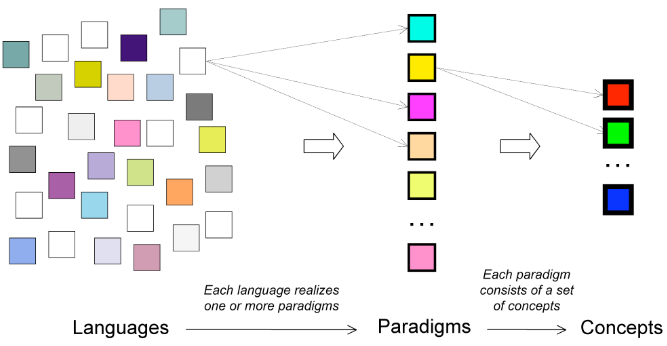
\includegraphics[width=\textwidth]{pictures/chapter1/intro-schema-langagues-paradigms.png}
    \caption{Schéma du concept de paradigme}
  \end{figure}

  \paragraph{}Dès lors, vu que \textbf{tous} les langages implémentent un ou des paradigmes, il suffit d'apprendre les
  principaux paradigmes pour avoir des connaisances de bases dans tous les langages existants et à venir.

  \tboxspace

  \begin{titletbox}{Définition formelle d'un paradigme}{success}
    \paragraph{}Un paradigme de programmation est une approche de programmation d'ordinateur basée sur un ensemble 
    cohérent de principes / règles ou des théories mathématiques.
    \tcblower
    \paragraph{} Un programme est écrit pour résoudre des problèmes
    \begin{itemize}[label=\textbullet, font=\small]
      \item Un programme réaliste doit savoir résoudre différents types de problèmes
      \item Chaque type de problème a besoin de son paradigme propre
      \item On a donc besoin de plusieurs paradigmes à combiner dans un même programme
    \end{itemize}
  \end{titletbox}


  \section{Étudier plusieurs paradigmes}

    \subsection{Comment étudier plusieurs paradigmes ?}

      \paragraph{}Comme la plupart des languages ne supportent qu'un paradigme et que nous devons apprendre plusieurs 
      d'entre eux, nous allons utiliser le langage de recherche Oz qui combinent plusieurs paradigmes avec sa propre 
      syntaxe et sémantique (un langage par paradigme étant beaucoup trop lourd pour un seul cours).
      Nous verrons aussi Erlang pour le paradigme \textit{actor dataflow programming}.

    \subsection{Combiner créer un programme multi-paradigmes ?}

      \begin{itemize}[label=\textbullet, font=\small]
        \item Chaque paradigme est une approche différente de pensée
        \item Un concept clé pour les implémenter est le {\color{danger} langage noyau}
      \end{itemize}

      \tboxspace

      \begin{titletbox}{Langage noyau}{success}
        Le langage noyau est à la base de tous les paradigmes. Celui fonctionne d'une manière simple, il contient les
        concepts essentiels auquel chaque paradigme va ajouter ses propres concepts un par un. De cette façon il est
        aussi facile de traduire un langage compliqué en langage noyau. En plus, les langages noyaux des différents
        paradigmes ont souvent beaucoup de concepts communs (exemple : conditions structurelles if/else, récursion, ...).
      \end{titletbox}

  \section{Paradigmes principaux}

      \paragraph{}Nous verrons dans ce cours les 5 paradigmes les plus importants. Il y existe bien sur plein d'autres
      pour d'autres types de problèmes (constraint programming, ...) que nous ne verrons pas ici.

      \tboxspace

      \begin{titletbox}{Paradigmes principaux}{info}
        \begin{itemize}[label=\textbullet, font=\small]
          \item Functional programming
          \item Object-orientied programming (Java)
          \item Functional dataflow programming
          \item Actor dataflow programming (multi-agent) (Erlang)
          \item Actives objects
        \end{itemize}
      \end{titletbox}

      \paragraph{} Ces paradigmes sont liés entre-eux comme le montre l'image ci-dessous (ils s'emboitent comme des 
      legos)

      \begin{figure}[H]
        \centering
        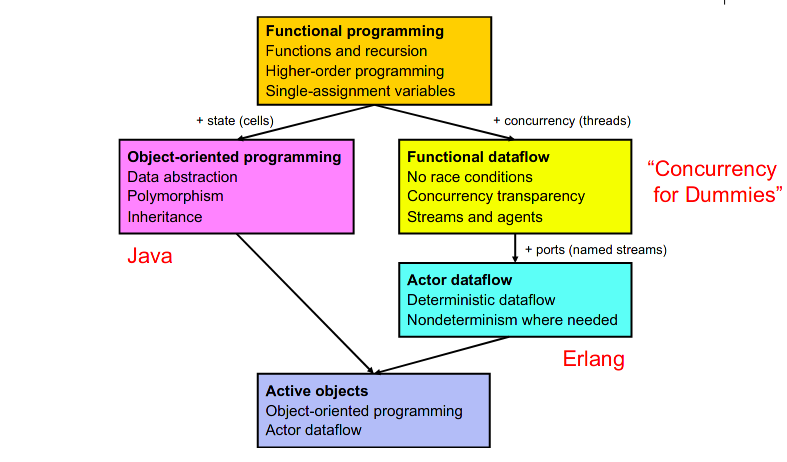
\includegraphics[width=\textwidth]{pictures/chapter1/five-paradigms.png}
        \caption{Liens entre les paradigmes}
      \end{figure}

      \section{Principes de base}

        % Concepts de base d'Oz -> slides 20 - 30 + voir si slides 31-35 pertinentes
